\begin{frame}[fragile]
  \frametitle{환경}
  \framesubtitle{Environments}
  \begin{itemize}
    \item \mintinline[escapeinside=||]{latex}{\begin{ENVNAME} ... \end{ENVNAME}} 꼴의 매크로를 모두 환경이라고 부릅니다. 
    \begin{itemize}
      \item 사실 이것은 \mintinline[escapeinside=||]{latex}{\ENVNAME ... \endENVNAME}로 정의됩니다.
    \end{itemize}
    \item 여러 중요한 환경들:
    \begin{itemize}
      \item \texttt{itemize}와 \texttt{enumerate} (with \texttt{enumitem})
      \item \texttt{matrix}
      \item \texttt{amsthm}
      \item \texttt{align}
      \item \texttt{figure}와 \texttt{center}
      \item \texttt{tabular}
    \end{itemize}
  \end{itemize}
\end{frame}

\begin{frame}[fragile]
  \frametitle{\texttt{itemize}와 \texttt{enumerate}}
  \framesubtitle{예시만 넣어 놓으면 택님께서 설명해 주실 거예요}
  \textbf{\texttt{enumitem} 패키지를 불러온 뒤},\vspace{-1em}
  \begin{minted}{latex}
\begin{itemize}
  \item 첫 번째
  \item[2] 두 번째
  \item[$\gamma$] wow
\end{itemize}

\begin{enumerate}[label={\roman*\arabic*}]
  \item 자동으로
  \item 올라가는
  \item 번호
\end{enumerate} 
  \end{minted}
\end{frame}

\begin{frame}[fragile]
  \frametitle{\texttt{matrix}}
  \framesubtitle{예시만 넣어 놓으면 택님께서 설명해 주실 거예요}
  \textbf{수식 모드 안에서}, \vspace{-1em}
  \begin{minted}{latex}
\begin{itemize}
\[ 
  \begin{pmatrix}
    a_{11} & a_{12} \\  
    a_{21} & a_{22}
  \end{pmatrix} \cdot
  \begin{bmatrix}
    b_{11} & b_{12} \\  
    b_{21} & b_{22}
  \end{bmatrix} =
  \begin{vmatrix}
    c_{11} & c_{12} \\  
    c_{21} & c_{22}
  \end{vmatrix} \cdot \mathbf I
\]
  \end{minted}
\end{frame}

\begin{frame}[fragile]
  \frametitle{\texttt{amsthm}}
  \framesubtitle{예시만 넣어 놓으면 택님께서 설명해 주실 거예요}
  \textbf{\texttt{amsthm} 패키지를 불러온 뒤},\vspace{-1em}
  \begin{minted}{latex}
\newtheorem{thm}{Theorem} % basic usagae
\newtheorem{lem}[thm]{Lemma} % shares the numbering w/ thm

\theoremstyle{definition}
\newtheorem{defn}{Definition}[section] % Def section.def_number

\theoremstyle{plain} % recover the theoremstyle
\newtheorem*{cor}{Corollary} % no numbering (*)

\begin{lem}[Lemma Name] This lemma is very awesome. \end{lem}
\begin{proof} Leave as an exercise. \end{proof}
  \end{minted}
\end{frame}

\begin{frame}[fragile]
  \frametitle{\texttt{figure}와 \texttt{center}}
  \framesubtitle{예시만 넣어 놓으면 택님께서 설명해 주실 거예요}
  \textbf{\texttt{float}, \texttt{graphicx}, (\texttt{adjustbox}) 패키지를 불러온 뒤},\vspace{-1em}
  \begin{minted}{latex}
% H means that it tries to put on the exact position
\begin{figure}[H] 
  \begin{center}
    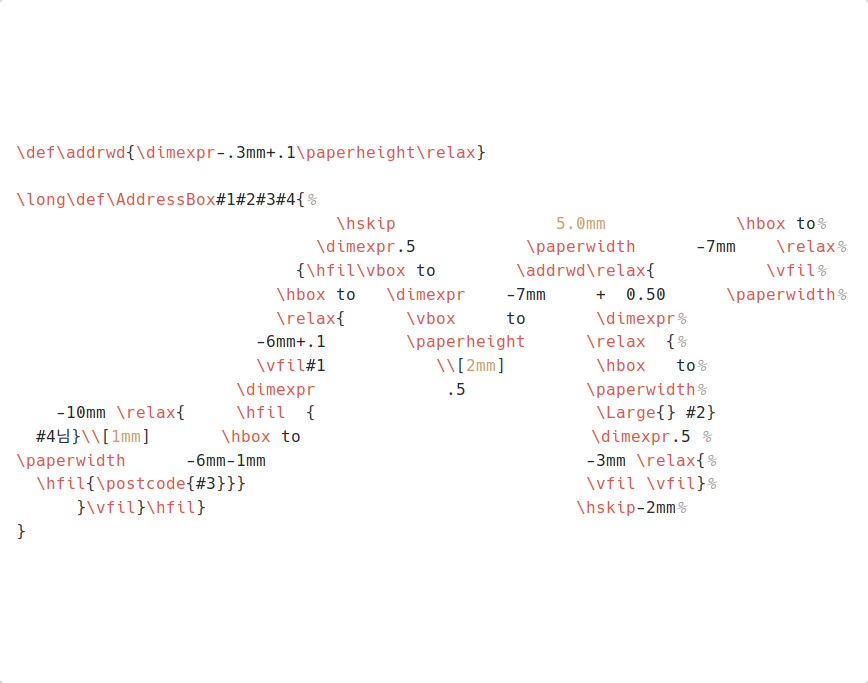
\includegraphics[width=0.5\textwidth]{msquare}
    \caption{Gorgeous}
  \end{center}
\end{figure}
  \end{minted}
\end{frame}

\begin{frame}[fragile]
  \frametitle{\texttt{tabular}}
  \framesubtitle{예시만 넣어 놓으면 택님께서 설명해 주실 거예요}
  \url{https://www.tablesgenerator.com/}
\end{frame}